%! Author = Len Washington III
%! Date = 9/14/2023

% Preamble
\documentclass[12pt]{report}

\usepackage[4]{cs430recitation}
\usepackage{algpseudocode}

% Document
\begin{document}

%<*Recitation-4>
\subsection{After Lecture 07 \& 08} -- Answer any questions on HW2 (due today)\\
Practice Problems (all taken from previous exams)
\begin{enumerate}[label=\arabic*.]
	\item Which one of the following is false?
	\begin{enumerate}[label=\choicelabel]
	    \item Heap sort is an in-place algorithm.
	    \item Heap sort has $O(n\log n)$ average case time complexity.
	    \item \answer{Heap sort is a stable sort.} Heap sort is an in-place algorithm as it needs $O(1)$ auxiliary space.
	    \item Heap sort is a comparison-based sorting algorithm.
	\end{enumerate}
	\item Consider the max heap shown below, the node with value 24 violates the max-heap property. Once heapify procedure is applied to it, which position will it be in?
	\begin{figure}[H]
		\centering
		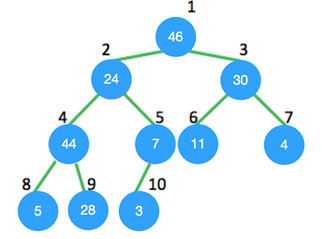
\includegraphics[width=0.5\textwidth]{rec4-heap}
		\label{fig:question-2}
	\end{figure}
	\begin{enumerate}[label=\choicelabel]
	    \item 5
		\item 8
		\item \answer{9}
		\item You cannot call heapify at the node with value 24
	\end{enumerate}
	\item Counting sort can be used on any numeric data.
	\begin{enumerate}[label=\choicelabel]
	    \item \answer{TRUE}, it can be used, but it is a very bad idea. Counting sort requires a very large range of numbers, counting sort requires a very large array. This reduces its memory efficiency and increases space consumption. So while it \emph{possible} to be used, it isn't a good idea to do so on any numeric data.
		\item FALSE
	\end{enumerate}
	\item Which of the following is not true about all comparison based sorting algorithms?
	\begin{enumerate}[label=\choicelabel]
	    \item The minimum possible runtime growth on a random input is $O(n\log n)$.
		\item Can be made stable by also using position when two elements are compared.
		\item Counting Sort is not a comparison-based sorting algorithm.
		\item Merge Sort is a comparison-based sorting algorithm.
	\end{enumerate}
	\item The BUILD-MAX-HEAP discussed in class and shown to be $O(n)$ uses this process. Call Heapify from heap index position $ \lfloor \frac{heapsize}{2} \rfloor$ down to heap index position 1. Building a heap can also be implemented by starting with an empty heap and repeatedly using MAX-HEAP-INSERT to insert the elements into the heap. Consider the following implementation:
	\begin{algorithm}[H]
		\label{alg:build-max-heap}
		\begin{algorithmic}[1]
		\Function{Build-Max-Heap1}{$A$}
			\State $H \gets $ empty heap (of max size $A.length$)
			\For{$i=1$ to $A.length$}
				\State $H.\Call{Max-Heap-Insert}{A[i]}$
			\EndFor
		\EndFunction
		\end{algorithmic}
	\end{algorithm}
	\begin{enumerate}[label=\choicelabel]
	    \item Do the procedures BUILD-MAX-HEAP and BUILD-MAX-HEAP1 always create the same heap when run on the same input array? Prove that they do, or provide a counterexample. \answer{The procedures do not always create the same heap when run on the same input array.}
		\item Show that in the worst case, BUILD-MAX-HEAP1 requires $\Theta(n\lg n)$ time to build an $n$-element heap. \answer{Since all but the last level is always filled, the height $h$ of an $n$ element heap is boundend because $\sum_{i=0}^{h} 2^{i}=2^{h+1}-1=\dots$ }
	\end{enumerate}
	\item The operation \Call{HEAP-DELETE}{$A$, $i$} deletes the item in node $i$ from heap $A$. Give an implementation of HEAP-DELETE that runs in $O(\lg n)$ time for an $n$-element max-heap.\answer{\begin{algorithm}[H]
			\caption{HEAP-DELETE}\label{alg:heap-delete}
			\begin{algorithmic}[1]
			\Function{HeapDelete}{$A$, $i$}
				\State swap A[i] with A[heapsize] \Comment{move the item to be deleted to the last position in the heap}
				\State decrement heapsize
				\State key $\gets$ A[$i$]
				\If{key $\leq$ A[\Call{Parent}{$i$}]}
					\State \Call{HEAPIFY}{$A$, $i$}
				\EndIf
				\State $\dots$
			\EndFunction
			\end{algorithmic}
		\end{algorithm}}
	\item Professor Fermat has the policy of giving A's to the top $n^{\frac{1}{2}}=\sqrt{n}$ students of his class, where $n$ is the number of students. The algorithm that he uses to determine the top $n^{\frac{1}{2}}$ students first sorts the list of students by their numerical, real-valued grade, and then picks the top $n^{\frac{1}{2}}$ students from the sorted list. This algorithm has time-complexity $O(n\log n)$ because of the sort. Can you suggest a more efficient algorithm that has time-complexity $O(n)$? Describe your algorithm informally in English and justify its time-complexity. \answer{You can use a MaxHeap to effectively sort the students based off of the students grades which takes $O(n)$. Now perform RemoveMax $\sqrt{n}$ times. Each RemoveMax operation takes time $O(\log N)$. Total time complexity of this algorithm is $O(n) + \log(n)\sqrt{n}=O(n)$ because $\log(n)\sqrt{n}=O(n)$, because $\log(n)=O\left( \sqrt{n} \right)$}
\end{enumerate}
%</Recitation-4>

\end{document}